\documentclass[12pt,letter]{article}
\usepackage[margin=1in]{geometry}
\usepackage[moduleName=SN76489]{KautenjaDSP}
% import a debugging package to show the margin boxes
% \usepackage{showframe}
% set the graphics path to the img directory
\graphicspath{{img/}}

% algorithm2e stuff
% \SetKwInOut{Objects}{$\CKmatrix{O}$}
% \SetKwInOut{Weights}{$\CKvector{w}$}

\begin{document}
\titlePage{SN76489-Logo}{SN76489-Module}{KautenjaDSP}

% -------------------
% MARK: Overview
% -------------------

\section{Overview}

SN76489 is an emulation of the Texas Instruments SN76489 audio processing unit from the Sega Master System for VCV Rack. The SN76489 chip contains three pulse waveform generators and a noise generator that selects between white-noise and periodic noise (LFSR).

SN76489 provides the key features of the SN76489 chip, namely,
\begin{itemize}
  \item \textbf{Triple pulse waveform generator:} Three 8-bit pulse waves with $50\%$ duty cycle and 10-bit frequency parameter
  \item \textbf{Noise generator:} Generate either white-noise or periodic noise at one of four shift rates: $N/512$, $N/1024$, $N/2048$, or the output of tone generator 3
  \item \textbf{4-bit Level Control:} 4-bit level control over each oscillator with mixer sliders and CV inputs
\end{itemize}

% -------------------
% MARK: Panel Layout
% -------------------

\clearpage
\section{Panel Layout}

\begin{figure}[!htp]
\centering
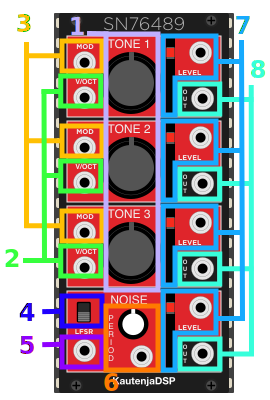
\includegraphics{SN76489-Manual}
\end{figure}

\begin{enumerate}
  \item Coarse frequency control over the four oscillators. Frequency is quantized to a 10-bit value for the tone generators.
  \item $V$/Octave inputs for pulse waveform generators.
  \item linear CV frequency modulation for pulse waveform generators.
  \item LFSR switch. When pointing down, the LFSR is enabled. When pointing up, the white-noise generator is active.
  \item CV LFSR gate, high at $2V$. Holds the LFSR generator as long as the input voltage is $>2V$. Inverts when LFSR switch is high.
  \item Noise generator shift rate. Select between one of four shift rates: the output of tone generator 3, $N / 512$, $N / 1024$, or $N / 2048$.
  \item Volume. Coarse amplitude control over the oscillators using the 4-bit amplifier. When no input is connected, the slider controls the level from $0\%$ to $100\%$. When an input is connected, the slider acts as an attenuator.
  \item Channel outputs, ${\approx}10V_{pp}$.
\end{enumerate}

% -------------------
% MARK: References
% -------------------

\clearpage
\renewcommand\refname{References \& Acknowledgments}
\nocite{*}
\bibliographystyle{apalike}
\bibliography{references}

\end{document}
